\documentclass[tikz,border=10pt]{standalone}
\usetikzlibrary{positioning,arrows.meta}
\definecolor{interfaceFill}{HTML}{B3E5FC}
\definecolor{interfaceBorder}{HTML}{0288D1}
\definecolor{classFill}{HTML}{EDE7F6}
\definecolor{classBorder}{HTML}{5E35B1}

\begin{document}
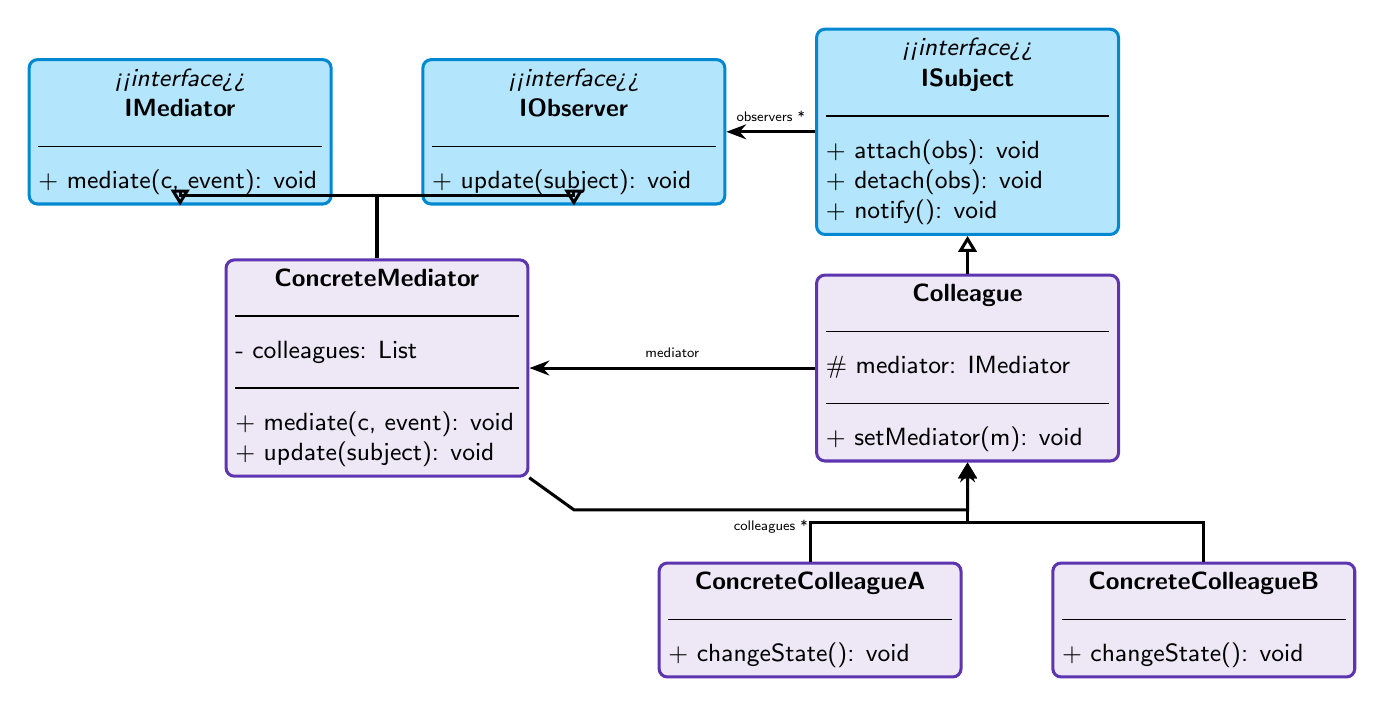
\begin{tikzpicture}[
    classBox/.style={
        rectangle, draw,
        minimum width=3.8cm, minimum height=1.2cm,
        align=left, rounded corners=3pt,
        line width=1.1pt, font=\sffamily\small
    },
    inheritance/.style={-{Triangle[open]}, line width=1.1pt},
    association/.style={-{Stealth[scale=0.9]}, line width=1.1pt}
]

  % Interfaces (Top Row)
  \node[classBox, fill=interfaceFill, draw=interfaceBorder] (IMediator) at (0, 3) {
    \makebox[3.6cm][c]{\itshape <<interface>>}\\
    \makebox[3.6cm][c]{\textbf{IMediator}}\\
    \vspace{2pt}\noindent\rule{3.6cm}{0.5pt}\vspace{2pt}\\
    + mediate(c, event): void
  };

  \node[classBox, fill=interfaceFill, draw=interfaceBorder] (IObserver) at (5, 3) {
    \makebox[3.6cm][c]{\itshape <<interface>>}\\
    \makebox[3.6cm][c]{\textbf{IObserver}}\\
    \vspace{2pt}\noindent\rule{3.6cm}{0.5pt}\vspace{2pt}\\
    + update(subject): void
  };

  \node[classBox, fill=interfaceFill, draw=interfaceBorder] (ISubject) at (10, 3) {
    \makebox[3.6cm][c]{\itshape <<interface>>}\\
    \makebox[3.6cm][c]{\textbf{ISubject}}\\
    \vspace{2pt}\noindent\rule{3.6cm}{0.5pt}\vspace{2pt}\\
    + attach(obs): void\\
    + detach(obs): void\\
    + notify(): void
  };

  % Concrete Mediator & Colleague (Middle Row)
  \node[classBox, fill=classFill, draw=classBorder] (ConcreteMediator) at (2.5, 0) {
    \makebox[3.6cm][c]{\textbf{ConcreteMediator}}\\
    \vspace{2pt}\noindent\rule{3.6cm}{0.5pt}\vspace{2pt}\\
    - colleagues: List\\
    \vspace{2pt}\noindent\rule{3.6cm}{0.5pt}\vspace{2pt}\\
    + mediate(c, event): void\\
    + update(subject): void
  };

  \node[classBox, fill=classFill, draw=classBorder] (Colleague) at (10, 0) {
    \makebox[3.6cm][c]{\textbf{\itshape Colleague}}\\
    \vspace{2pt}\noindent\rule{3.6cm}{0.5pt}\vspace{2pt}\\
    \# mediator: IMediator\\
    \vspace{2pt}\noindent\rule{3.6cm}{0.5pt}\vspace{2pt}\\
    + setMediator(m): void
  };

  % Concrete Colleagues (Bottom Row)
  \node[classBox, fill=classFill, draw=classBorder] (ColleagueA) at (8, -3.2) {
    \makebox[3.6cm][c]{\textbf{ConcreteColleagueA}}\\
    \vspace{2pt}\noindent\rule{3.6cm}{0.5pt}\vspace{2pt}\\
    + changeState(): void
  };

  \node[classBox, fill=classFill, draw=classBorder] (ColleagueB) at (13, -3.2) {
    \makebox[3.6cm][c]{\textbf{ConcreteColleagueB}}\\
    \vspace{2pt}\noindent\rule{3.6cm}{0.5pt}\vspace{2pt}\\
    + changeState(): void
  };

  % Inheritance / Realization lines
  \draw[inheritance] (ConcreteMediator.north) -- ++(0, 0.8) -| (IMediator.south);
  \draw[inheritance] (ConcreteMediator.north) -- ++(0, 0.8) -| (IObserver.south);
  \draw[inheritance] (Colleague) -- (ISubject);
  
  \draw[inheritance] (ColleagueA.north) -- ++(0, 0.5) -| (Colleague.south);
  \draw[inheritance] (ColleagueB.north) -- ++(0, 0.5) -| (Colleague.south);

  % Associations
  \draw[association] (Colleague.west) -- (ConcreteMediator.east)
      node[midway, above, font=\sffamily\tiny] {mediator};
      
  \draw[association] (ConcreteMediator) -- ++(2.5, -1.8) -| (Colleague.south)
      node[pos=0.25, below, font=\sffamily\tiny] {colleagues *};

  % ISubject to IObserver link (aggregate/association)
  \draw[association] (ISubject) -- (IObserver)
      node[midway, above, font=\sffamily\tiny] {observers *};

\end{tikzpicture}
\end{document}
